%\newpage

\section{Instrumente und Samples}

In diesem Kapitel wird erklärt, was der Unterschied zwischen so genannten sampled und unsampled Songs ist, wie einzelne Instrumente definiert werden, was Sample Groups sind und wie wir eigene Samples erstellen und einbinden können. \\
Außerdem benötigen wir für das Kapitel folgende Programme:

\medskip

\begin{itemize}
	\item Audacity
	\item OpenMPT
	\item BRRPlayer von Vitor Vilela
	\item BRRTools von Bregalad und nyanpasu64 oder das C700 VST Plugin
\end{itemize}

\medskip


Unsampled Songs sind Songs, die ausschließlich Samples aus SMW benutzen. Ein Beispiel für ein unsampled Song ist der von uns erstellt Song aus Kapitel \ref{sec:ErstenSongSchreiben}. \\
Von sampled Songs ist die Rede, sobald mindestens ein custom Sample (ein Sample, dass aus einem anderen Spiel kommt oder selbst erstellt wurde) für den Song verwendet wird. \\
Unsampled Songs klingen oft nach SMW und haben den Vorteil, dass sie nur wenig Platz im Audio RAM einnehmen. Dafür ist man jedoch stark eingeschränkt in der Instrumentauswahl. Sampled Songs haben dieses Problem nicht, können aber schnell den gesamten Arbeitsspeicher belegen, weswegen besonders auf den Speicherplatz geachtet werden muss.

\subsection{Custom Samples}

Der SPC700 arbeitet mit so genannten .brr Samples (Bit Rate Reduction). Es gibt verschiedene Möglichkeiten an diese Samples zu gelangen:

\medskip

\begin{itemize}
	\item Ein Sample Pack herunterladen
	\item Samples aus einer SPC Datei extrahieren, z.B. mit split700, dem C700 Plugin oder SPC2MML
	\item Ein Sample aus einer .wav Datei selbst erstellen 
\end{itemize}

\medskip

Ein sehr umfangreiches Sample Pack ist samples of insanity von musicalman. Es ist hier verfügbar:
\href{https://bin.smwcentral.net/u/29022/soi-2019-07-12.zip}{https://bin.smwcentral.net/u/29022/soi-2019-07-12.zip}

\bigskip

Sollen Custom Samples für einen Song verwendet werden, müssen diese in einem Unterverzeichnis von AddmusicK/samples/ liegen. Am besten legt man für jeden Song einen eigenen Ordner für Samples an. Mit dem Spezial Befehl \#path weiß AddMusicK, in welchem Verzeichnis Samples gesucht werden sollen. \\
Wir fügen am Beispiel unseres Songs aus Kapitel \ref{sec:ErstenSongSchreiben} ein Custom Sample ein. Als erstes erstellen wir einen Ordner mit dem Namen \textit{Prelude} in AddmusicK/samples/. Danach kopieren wir uns das Sample Harp 2.brr, welches in samples of insanity/individual samples/other liegt und fügen es in den von uns zuvor erstellten Ordner \textit{Prelude} ein. Außerdem öffnen wir das beiliegende Textdokument \textit{!patterns.txt} worauf wir gleich noch zurückgreifen werden. \\
Jetzt öffnen wir wieder unseren Song und geben den Pfad mit \#path  \dq Prelude\dq{} an. Danach bestimmen wir mit \#samples\{\}, welche Samples aus dem Ordner benutzt werden sollen. Wir tragen neben dem Samplenamen noch eine Samplegroup ein die wir verwenden möchten, was entweder die Samplegroup \#default oder \#optimized ist, falls wir keine eigene erstellen. \\
AddMusicK legt im Hintergrund die Samplegroup \#default automatisch an wenn kein \#Samples\{\} Block vorhanden ist, weswegen wir bisher keine Samplegroup selber anlegen mussten.


\medskip

\lstinputlisting[framexleftmargin=8mm, frame=shadowbox, rulesepcolor=\color{blue}, numbers=left, firstline=1, lastline=9]{codes/Samples.txt}

\medskip

Als letztes definieren wir uns das neue Instrument. Wir ersetzen dafür das alte Instrument an die Position @30, indem  die gesamte Zeile gelöscht wird und dafür der Samplename plus den ersten 5 Hexwerten aus  \textit{!patterns.txt} die hinter  \textit{harp 2.brr} stehen. \\
Der Anfang des Songs sollte nun wie folgt aussehen:

\medskip

\lstinputlisting[framexleftmargin=8mm, frame=shadowbox, rulesepcolor=\color{blue}, numbers=left, firstline=1, lastline=17]{codes/Samples.txt}

\medskip


\subsection{Instrumente definieren}

Möglicherweise möchten wir ein Instrument in seinen Eigenschaften ändern oder haben gar keine Standardwerte, weil wir das Sample beispielsweise selbst erstellt haben. Was es mit den einzelnen Hexwerten auf sich hat wird im Folgenden erklärt.\\

\medskip
 
\lstinputlisting[framexleftmargin=8mm, frame=shadowbox, rulesepcolor=\color{blue}, numbers=left, firstline=13, lastline=13]{codes/Samples.txt}
 
\medskip

Als erstes wird entweder die Nummer des SMW Samples oder der Custom Sample Name angegeben, der definiert werden soll.
Danach beschreiben die Hexwerte der Reihe nach: \\
Attack und Decay (AD), Sustain und Release (SR), Gain, Pitch, Fine Pitch.

\bigskip

ADSR und Gain beschreiben die Hüllkurve bzw. Anschlags- und Abklingverhalten des Instruments, wobei immer nur ADSR oder Gain gleichzeitig aktiv ist. Es ist aber möglich, mit weiteren Befehlen zwischen ADSR und Gain zu wechseln und auch die  Werte zu verändern. \\
Mit Pitch und Fine Pitch stimmen wir das Instrument auf den richtigen Pitch, ähnlich wie eine Gitarre. Soll das Instrument um eine Oktave vergrößert oder verkleinert werden, müssen Pitch und Fine Pitch verdoppelt bzw. halbiert werden.


\subsubsection{ADSR}

Allgemein lassen sich verschiedene Parameter mit ADSR ansteuern, im Falle von AddMusicK allerdings nur der Verlauf der Lautstärke. Außerdem ist ADSR in AddMusicK leicht anders definiert als üblich. Das kommt daher, dass es beim SPC700 kein echtes Release Event gibt. Zwar gibt es so genannte Off Keying Events (immer wenn eine Note endet), diese lösen aber nicht das herkömmliche Release Event aus, weil das Instrument sofort aufhört zu spielen, sobald das Off Keying Event eintritt. (Es gibt allerdings die Möglichkeit, ein künstliches Release Event nach Ende einer Note selbst zu erzeugen)

\bigskip

Die 4 Parameter beschreiben hier folgende Eigenschaften:

\medskip

\begin{itemize}
	\item \textbf{Attack (Anstieg)} -- gibt die Dauer an, bis die Lautstärke das Maximum erreicht hat.
	\item \textbf{Decay (Abfall)} -- gibt die Dauer an, die zwischen Maximum und Sustain Wert liegt.
	\item \textbf{Sustain (Halten)} -- gibt das Verhältnis zwischen abfallenden Wert nach der Decay Dauer und dem Maximum an.
	\item \textbf{Release (Loslassen)} -- gibt die Dauer an, bis die Lautstärke 0 erreicht.
\end{itemize}


\bigskip

\begin{figure}[htbp] \centering
	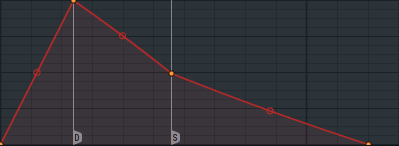
\includegraphics[width=.95\linewidth]{images/ADSR.png}
	\caption{ADSR}
	\label{ADSR}
\end{figure}

\begin{table}
\begin{tabularx}{\textwidth}{|l|X|X|X|X|X|}
	\hline
	Wert & Attack (Sek.) & Decay (Sek.)  & Sustain (Verhältnis) & Release (Sek.) Wert $\leq$ F & Release (Sek.) Wert $>$ F \\
	\hline
	00 & 4.1 & 1.2 (\$ED) & 1/8 & Unendlich & 1.2\\
	\hline
	01 & 2.6 & 0.74 (\$ED) & 1/8 & 38 & 0.88 \\
	\hline
	02 & 1.5 & 0.44 (\$ED) & 2/8 & 28 & 0.74 \\
	\hline
	03 & 1.0 & 0.29 (\$ED) & 2/8 & 24 & 0.59 \\
	\hline
	04 & 0.64 & 0.18 (\$ED) & 3/8 & 19 & 0.44 \\
	\hline
	05 & 0.38 & 0.11 (\$ED) & 3/8 & 14 & 0.37 \\
	\hline
	06 & 0.26 & 0.074 (\$ED) & 4/8 & 12 & 0.29 \\
	\hline
	07 & 0.16 & 0.037 (\$ED) & 4/8 & 9.4 & 0.22 \\
	\hline
	08 & 0.096 & 1.2 & 5/8 & 7.1 & 0.18 \\
	\hline
	09 & 0.064 & 0.74 & 5/8 & 5.9 & 0.15 \\
	\hline
	0A & 0.04 & 0.44 & 6/8 & 4.7 & 0.11 \\
	\hline
	0B & 0.024 & 0.29 & 6/8 & 3.5 & 0.092 \\
	\hline
	0C & 0.016 & 0.18 & 7/8 & 2.9 & 0.074 \\
	\hline
	0D & 0.01 & 0.11 & 7/8 & 2.4 & 0.055 \\
	\hline
	0E & 0.006 & 0.074 & 1 & 1.8 & 0.037 \\
	\hline
	0F & 0 & 0.037 & 1 & 1.5 & 0.018 \\
	\hline
\end{tabularx}
\label{tab:ADSR}
\caption{ADSR Werte}
\end{table}

\bigskip

Die Tabelle und die beiden unterschiedlichen Befehle zur ADSR Beschreibung benötigen eine genauere Erklärung. Diese erfolgt am Beispiel unseres Custom Instruments.


\medskip

\lstinputlisting[framexleftmargin=8mm, frame=shadowbox, rulesepcolor=\color{blue}, numbers=left, firstline=1, lastline=5]{codes/ADSR.txt}

\medskip

Beide Befehle beschreiben die gleichen ADSR Werte. Als erstes sei gesagt, dass die Reihenfolge der ADSR Werte nicht \$AD \$SR, sondern \$DA \$SR entspricht. \\
Als nächstes fällt auf, dass sich der Decay Wert unterscheidet. Der Decay Wert in \#instruments\{\} muss immer um 8 aufaddiert werden. \\
Sustain und Release Werte hängen voneinander ab. In diesem Beispiel ist die Release Dauer nicht unendlich, obwohl der Release Wert auf 0 steht. Für eine Release Dauer von unendlich muss der Sustain Wert immer eine gerade Zahl sein. Hier müsste der Sustain Wert auf A gesetzt werden, damit das Sustain Verhältnis gleich bleibt, die Release Dauer aber unendlich beträgt. \\
Falls \$DA in \#instruments\{\} kleiner als \$80 ist, wird automatisch Gain aktiviert. Genauso wird Gain aktiviert, falls im \$ED Befehl der \$DA Wert $\geq 80$ ist.

\bigskip

Das Instrument wird durch ADSR wie folgt beschrieben: \\
\textbf{Attack:} 0 Sek. \\
\textbf{Decay:} 0.29 Sek. \\
\textbf{Sustain:} 6/8 vom Maximum \\
\textbf{Release:} 1.2 Sek.



\subsubsection{Gain}

Neben ADSR kann ein Instrument auch durch Gain beschrieben werden. Wie bei ADSR gibt es zwei Möglichkeiten, Gain zu definieren. Zum einen durch das dritte Argument in \#instruments\{\} (wird dort aber nur aktiv, falls \$DA in \#instruments\{\} kleiner als \$80 ist), zum anderen durch die Hexbefehle \$FA \$01 \$XX oder \$ED \$80+ \$XX. \\
Gain beschreibt keine vollständige Hüllkurve sondern nur das Anschlag- oder Abklingverhalten eines Instruments. Im Vergleich zu ADSR bietet Gain allerdings auch exponentielle Verläufe an, wohingegen durch ADSR nur lineare Verläufe möglich sind. \\
Es gibt fünf verschiedene Gain Modi:

\medskip

\begin{itemize}
	\item \textbf{Direct}
	\item \textbf{Decrease}
	\item \textbf{Exponential Decrease}
	\item \textbf{Increase}
	\item \textbf{Bent Line Increase}
\end{itemize}


\bigskip

Bei Gain Werten zwischen 00 bis 7F ist der Modus Direct aktiv (direkter Anschlag).
Die weiteren Modi inklusive Anstiegs- und Abklingszeiten stehen in der folgenden Tabelle:

\bigskip

\begin{table}[htbp]
\begin{tabularx}{\textwidth}{|X|X|}
	\hline
	Zeit von Wert 7F bis 0: & Zeit von Wert 0 bis 7F: \\
	\hline
\end{tabularx}

\begin{tabularx}{\textwidth}{|l|X|l|X|l|X|l|X|}
	\hline
	Wert & Decrease & Wert & Exp Decrease & Wert & Increase & Wert & Bent Line Increase \\
	\hline
	80 & Unendlich & A0 & Unendlich & C0 & Unendlich & E0 & Unendlich \\
	\hline
	81 & 4.1 s & A1 & 38 s & C1 & 4.1 s & E0 & 7.2 s \\
	\hline
	82 & 3.1 s & A2 & 28 s & C2 & 3.1 s & E2 & 5.4 s \\
	\hline
	83 & 2.6 s & A3 & 24 s & C3 & 2.6 s & E3 & 4.6 s \\
	\hline
	84 & 2.0 s & A4 & 19 s & C4 & 2.0 s & E4 & 3.5 s \\
	\hline
	85 & 1.5 s & A5 & 14 s & C5 & 1.5 s & E5 & 2.6 s \\
	\hline
	86 & 1.3 s & A6 & 12 s & C6 & 1.3 s & E6 & 2.3 s \\
	\hline
	87 & 1.0 s & A7 & 9.4 s & C7 & 1.0 s & E7 & 1.8 s \\
	\hline
	88 & 770 ms & A8 & 7.1 s & C8 & 770 ms & E8 & 1.3 s \\
	\hline
	89 & 640 ms & A9 & 5.9 s & C9 & 640 ms & E9 & 1.1 s \\
	\hline
	8A & 510 ms & AA & 4.7 s & CA & 510 ms & EA & 900 ms \\
	\hline
	8B & 380 ms & AB & 3.5 s & CB & 380 ms & EB & 670 ms \\
	\hline
	8C & 320 ms & AC & 2.9 s & CC & 320 ms & EC & 560 ms \\
	\hline
	8D & 260 ms & AD & 2.4 s & CD & 260 ms & ED & 450 ms \\
	\hline
	8E & 190 ms & AE & 1.8 s & CE & 190 ms & EE & 340 ms \\
	\hline
	8F & 160 ms & AF & 1.5 s & CF & 160 ms & EF & 280 ms \\
	\hline
	90 & 130 ms & B0 & 1.2 s & D0 & 130 ms & F0 & 220 ms \\
	\hline
	91 & 96 ms & B1 & 880 ms & D1 & 96 ms & F1 & 170 ms \\
	\hline
	92 & 80 ms & B2 & 740 ms & D2 & 80 ms & F2 & 140 ms \\
	\hline
	93 & 64 ms & B3 & 590 ms & D3 & 64 ms & F3 & 110 ms \\
	\hline
	94 & 48 ms & B4 & 440 ms & D4 & 48 ms & F4 & 84 ms \\
	\hline
	95 & 40 ms & B5 & 370 ms & D5 & 40 ms & F5 & 70 ms \\
	\hline
	96 & 32 ms & B6 & 290 ms & D6 & 32 ms & F6 & 56 ms \\
	\hline
	97 & 24 ms & B7 & 220 ms & D7 & 24 ms & F7 & 42 ms \\
	\hline
	98 & 20 ms & B8 & 180 ms & D8 & 20 ms & F8 & 35 ms \\
	\hline
	99 & 16 ms & B9 & 150 ms & D9 & 16 ms & F9 & 28 ms \\
	\hline
	9A & 12 ms & BA & 110 ms & DA & 12 ms & FA & 21 ms \\
	\hline
	9B & 10 ms & BB & 92 ms & DB & 10 ms & FB & 18 ms \\
	\hline
	9C & 8 ms & BC & 74 ms & DC & 8 ms & FC & 14 ms \\
	\hline
	9D & 6 ms & BD & 55 ms & DD & 6 ms & FD & 11 ms \\
	\hline
	9E & 4 ms & BE & 37 ms & DE & 4 ms & FE & 7 ms \\
	\hline
	9F & 2 ms & BF & 18 ms & DF & 2 ms & FF & 3.5 ms \\
	\hline
\end{tabularx}
\caption{Gain Table von ggamer77}
\end{table}

\medskip

Decrease und Exponential Decrease werden nur wirksam, wenn sie während einer gespielten Note aktiviert wird. Dies können wir mittels Haltebogen erreichen.

\bigskip

Im SPC700 Player werden die einzelnen Modi wie folgt angezeigt: 

\bigskip

\begin{tabularx}{\textwidth}{l l}
Direct & 
\textcolor{blue}{Ga}
\textcolor{red}{D}
- -
\\
Decrease & 
\textcolor{blue}{Ga}
\textcolor{green}{A}
0 0
\\
Exponential Decrease & 
\textcolor{blue}{Ga}
\textcolor{green}{A}
0
\textcolor{red}{1}
\\
Increase &
\textcolor{blue}{Ga}
\textcolor{green}{A}
\textcolor{red}{1}
0
\\
Bent Line Increase &
\textcolor{blue}{Ga}
\textcolor{green}{A}
\textcolor{red}{1}
\textcolor{red}{1}
\end{tabularx}

\bigskip

Die geänderten ADSR Werte durch \$ED bzw. Gain Wert durch \$FA \$01 oder \$ED werden mit erneutem Aufrufen des Instruments (@) wieder zurückgesetzt.

\subsection{Sample Groups}

Wer bereits häufiger Musik in eine Rom gepatcht oder sampled Songs selbst geschrieben hat, wird wahrscheinlich schon auf Sample Groups gestoßen sein. \\
Sample Groups sind -- wie der Name schon vermuten lässt -- eine vordefinierte Gruppe an Samples. AddMusicK stellt die Sample Groups \#default und \#optimized zur Verfügung. Diese beinhalten alle SMW Samples, die für Local Songs (normale Hintergrundmusik), Global Songs (Hintergrundmusik, die in allen Leveln geladen sind, z.B. Stage Clear oder P-Block) und Soundeffekte verwendet werden.
Sie befinden sich in \textit{samples/default/} bzw. \textit{samples/optimized/}.

\bigskip

Sofern kein \#samples\{\} Block verwendet wird, setzt AddMusicK versteckt die Sample Group \#default. Sobald \#samples\{\} benutzt wird, muss eine Sample Group gesetzt werden.
Ohne Sample Group wird nur das Standardinstrument @0 geladen, alle anderen SMW Samples können dann nicht mehr verwendet werden. \\
In eine Rom gepatcht hat dies außerdem zur Folge, dass weder Global Songs noch Soundeffekte richtig abgespielt werden. Das liegt daran, dass jeder Soundeffekt in SMW aus den gleichen Samples erzeugt werden, die auch für die Musikinstrumente benutzt werden.
Stattdessen werden Custom Samples die im \#samples\{\} Block liegen verwendet. Sobald ein sampled Song geschrieben wird, muss also eine Sample Group gesetzt werden.

\bigskip

Bei der Sample Group \#default handelt es sich um die original SMW Samples, die Samples aus \#optimized beinhalten nur die Hälfte der Informationen, wodurch diese auch nur halb so groß sind.
Der Informationsverlust bedeutet eine geringere Soundqualität, diese ist aber kaum wahrnehmbar. Die Wahl der Sample Group hängt also nur davon ab, wie viel freier Speicher noch im Arbeitsspeicher vorhanden ist.

\subsubsection*{Custom Sample Groups}

Es ist auch möglich eine eigene Sample Group anzulegen. Hauptmotivation ist, etwas Arbeitsspeicher einzusparen, indem einzelne Samples aus der Sample Group durch die Datei \textit{EMPTY.brr} ersetzt werden. Dabei handelt es sich um ein Sample ohne Informationen und dient nur als Platzhalter, damit alle anderen Samples ihre richtige Position in der Liste beibehalten.

\bigskip

In \textit{Addmusic\_sample groups.txt} werden alle Sample Groups definiert. Zwei Dinge fallen auf: Zum einen scheint es, als würden Samples fehlen. Die Samples @11, @16, @18, @23 - @28 werden jedoch nur durch die Samples aus der Liste erzeugt, die aber andere ADSR Einstellungen besitzen. \\

Zum anderen stehen hinter den Samples @14, @17 und @21 keine Ausrufezeichen. Ein Ausrufezeichen hinter einem Samplenamen bewirkt, dass diese global (also dauerhaft) geladen sind, solange die Sample Group verwendet wird. Die Samples @14, @17 und @21 sind die einzigen Samples, die weder für Global Songs, noch Soundeffekte und ausschließlich für einige Local Songs verwendet werden und daher nicht global geladen werden müssen. \\
Unter \href{https://www.smwcentral.net/?p=viewthread\&t=97787}{https://www.smwcentral.net/?p=viewthread\&t=97787} ist eine vollständige Liste, welche Samples für welche Soundeffekte und Global Songs verwendet werden. \\
Die populärsten Samples die durch \textit{EMPTY.brr} ersetzt werden sind \textit{12 SMW @15.brr} (wird nur für Yoshi Sound verwendet), \textit{09 SMW @7.brr} (wird nur für den Global Song Bonus End verwendet) und \textit{13 SMW Thunder.brr}. Eine Sample Group ohne \textit{12 SMW @15.brr} wäre daher nicht kompatibel mit Leveln, die Yoshi benutzen. Daher muss immer darauf hingewiesen werden, welche Sounds oder Global Songs nicht mehr funktionieren, wenn man einen Song teilt oder hochlädt.

\bigskip

Falls eine neue Sample Group angelegt werden soll, kopiert man dafür am einfachsten die Sample Group \#optimized aus \textit{Addmusic\_sample groups.txt}, fügt diese im Textdokument ein mit einem anderen Namen als optimized und ersetzt Samples, die nicht verwendet werden sollen durch \textit{\dq EMPTY.brr\dq{}!}. Im Song selbst wird die Sample Group schließlich mit \#SampleGroupName geladen.

\subsection{Eigene Samples erstellen}


Jede Audioquelle, die sich in eine .wav Datei konvertieren lässt, sind potentielle Samples die sich in Songs benutzen lassen. Als erstes öffnen wir Audacity und laden unsere Sounddatei ein
(z.B. .mp3 oder .wav). Mit dem Selection Tool (\textit{F1}) markieren wir nun alle Bereiche, die entfernt werden sollen und löschen diese mit \textit{Entf}. Danach klicken wir links auf den kleinen Pfeil neben dem Dateinahmen und wählen dort \textit{Split Stereo to Mono} aus.

\begin{figure}[htbp] \centering
	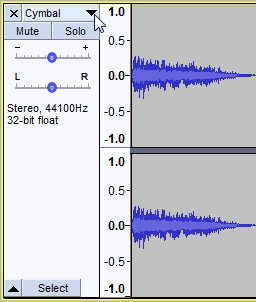
\includegraphics[width=.50\linewidth]{images/Audacity.png}
	\caption{Track aufteilen in Audacity}
	\label{Audacity}
\end{figure}

\bigskip

Dadurch beugen wir vor, dass das Sample im nächsten Schritt nicht nur auf einem Lautsprecher zu hören ist. Außerdem wird dadurch die Größe des Samples ungefähr halbiert. \\
Es ist auch möglich, 2 Stereo Samples zu erzeugen. Dafür muss \textit{Split Stereo Track} anstatt \textit{Split Stereo to Mono} ausgewählt werden. Das hat allerdings den Nachteil, dass 2 Samples für einen Sound benötigt werden, was wiederum bedeutet, dass doppelt so viel Speicher verbraucht wird und im Song selbst 2 Kanäle belegt werden müssen.

\bigskip

Die Datei wird nun als .wav Datei exportiert mit einer Signed 16-bit PCM Codierung.

%\bigskip

\subsubsection*{OpenMPT}

Als nächstes öffnen wir OpenMPT, laden unsere exportierte .wav ein und klicken oben auf den Reiter \textit{Samples}. Es öffnet sich folgendes Fenster:

\begin{figure}[htbp] \centering
	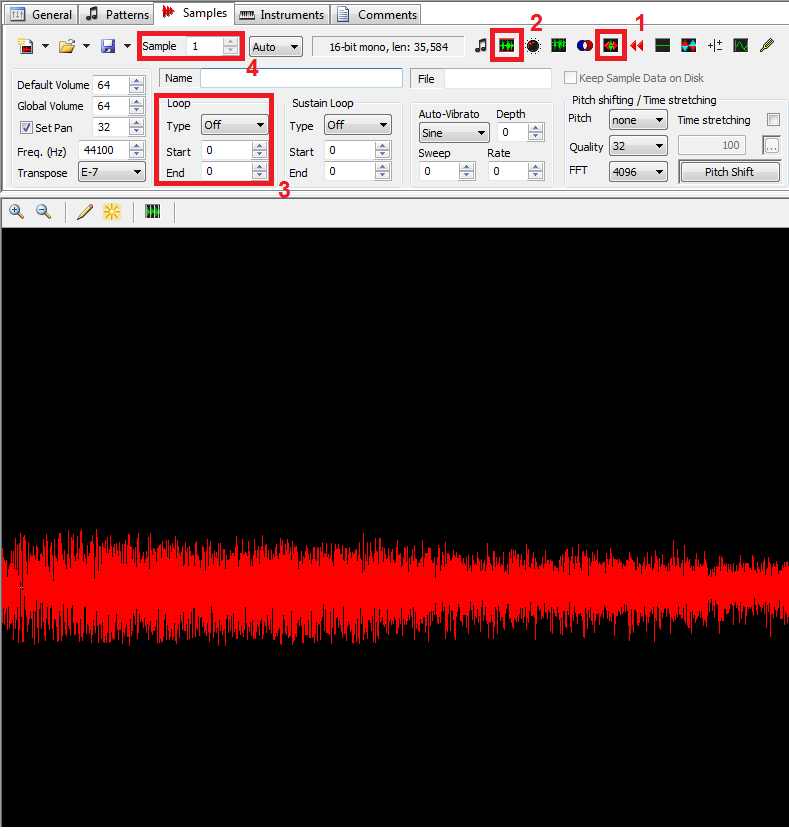
\includegraphics[width=.95\linewidth]{images/OpenMTP.png}
	\caption{Samples bearbeiten in OpenMPT}
	\label{OpenMTP}
\end{figure}

\bigskip

Wir benötigen nur die 4 markierten Funktionen. Diese sind:

\medskip

\begin{itemize}
	\item \textbf{1. Up-/Down Sampling}
	\item \textbf{2. Normalize}
	\item \textbf{3. Loop Points}
	\item \textbf{4. Sample Auswahl} 
\end{itemize}

\medskip

Punkt 1 benutzen wir zum Downsamplen. Damit ist gemeint, dass die Samplerate -- also die Abtastrate -- verringert wird. Voreingestellt ist eine Samplerate von 44.1 kHz, halbieren wir diese durch downsamplen auf 22.05 kHz wird unser Signal nur noch mit der halben Anzahl an Samples (damit sind die Abtastpunkte gemeint) abgetastet. Die Konsequenzen sind, dass die Hälfte an Informationen gelöscht werden, was in ein halb so großes Signal mit Qualitätsverlust resultiert. Außerdem wird die akustisch wahrnehmbare Frequenz bei gleichem Pitch verdoppelt was wir an anderer Stelle ausnutzen können. \\
In der Regel sollte man ein- bis maximal zweimal downsamplen um das Sample klein genug zu bekommen.

\bigskip

Punkt 2 verstärkt unser gesamtes Sample im gleichen Maß ohne Clipping zu erzeugen (Abschneiden der Amplitude). Es ist immer einfacher, ein Sample im nachhinein leiser einzustellen als lauter, weshalb wir diese Option immer benutzen sollten.

\bigskip

Punkt 3 benötigen wir nur für Samples die loopen, also unendlich lang zu hören sind, solange eine Note nicht aufhört zu spielen.  Dieser Punkt ist recht anspruchsvoll, da es nicht einfach ist, Start und Endpunkte zu finden, die ein Sample sauber loopen zu lassen. Besonders bei stark heruntergesampleten Signalen fängt ein Sample schnell an zu \dq schwingen\dq{}. \\
Wichtig hierbei ist, dass beide Looppunkte ein vielfaches von 16 sein müssen, falls wir im nächsten Schritt zum Konvertieren ein anderes Programm als BRRTools oder das C700 Plugin benutzen sollten. \\
Sustain Loop benötigen wir nicht. Dieses beschreibt einen Loop der verlassen wird, sobald das Sample nicht mehr gespielt wird und dadurch das Ende zu hören ist. Da es kein echtes Release Event in AddMusicK gibt und ein Sample mit Ende einer Note sofort aufhört zu spielen, kann in einem geloopten Sample der Rest des Signals hinter dem End Loop Punkt gelöscht werden, weil dieses nie erreicht wird.


\bigskip

Punkt 4 wird nur benötigt, falls wir vorher in Audacity das Sample auf 2 Stereo Tracks aufgeteilt haben. Hier kann zwischen den einzelnen Samples hin und her gewechselt werden.

\bigskip

Ist das Sample fertig bearbeitet, kann es über das Diskettensymbol neben Punkt 4 wieder als .wav Datei gespeichert werden. \\
Als letzten Schritt muss die .wav Datei nur noch in eine .brr Datei konvertiert werden. Dafür benutzen wir entweder das C700 Plugin (bevorzugt) oder BRRTools.

\subsubsection*{C700}

Das C700 Plugin muss in eine DAW (Digital Audio Workstation) unserer Wahl installiert werden. Unter anderem unterstützen FL Studio, LMMS und OpenMPT das Plugin. \\
Wir öffnen das Plugin in unserer DAW und legen per \textit{Drag \& Drop} die .wav Datei in die Mitte des Plugins. Danach klicken wir auf \textit{Save Smpl...} woraufhin das Plugin eine .brr und eine .smpl Datei erstellt. Letztere kann gelöscht werden. Das erstellte .brr Sample kann nun über den \#samples\{\} Block in einen Song geladen werden.

\begin{figure}[htbp] \centering
	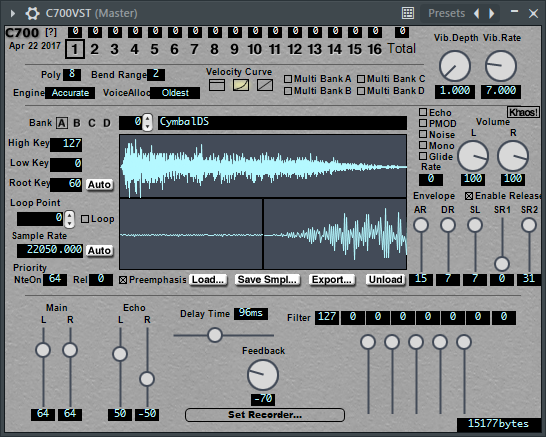
\includegraphics[width=.95\linewidth]{images/C700.png}
	\caption{C700 VST Plugin in FL Studio}
	\label{C700}
\end{figure}

\subsubsection*{BRRTools}

Alternativ zu C700 kann auch BRRTools verwendet werden. BRRTools kommt mit 3 konsolenbasierten Programmen daher. Wir benötigen \textit{brr\_encoder.exe}. Zunächst legen wir das Sample in das gleiche Verzeichnis wie \textit{brr\_encoder.exe}, danach öffnen wir die Konsole und navigieren in das selbige Verzeichnis und geben folgendes ein:

\bigskip

\textit{brr\_encoder Samplename.wav Samplename.brr}

\bigskip

\begin{figure}[htbp] \centering
	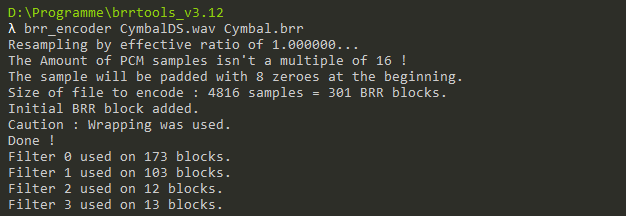
\includegraphics[width=.95\linewidth]{images/BRRTools.png}
	\caption{brr encoder über die Konsole starten}
	\label{BRRTools}
\end{figure}

Hinter \textit{brr\_encoder} können verschiedene Optionen hinzugefügt werden. Diese und weitere Erklärungen finden sich in der ReadMe.

\newpage
